\clearpage

\begin{figure}[h!]
    \centering
    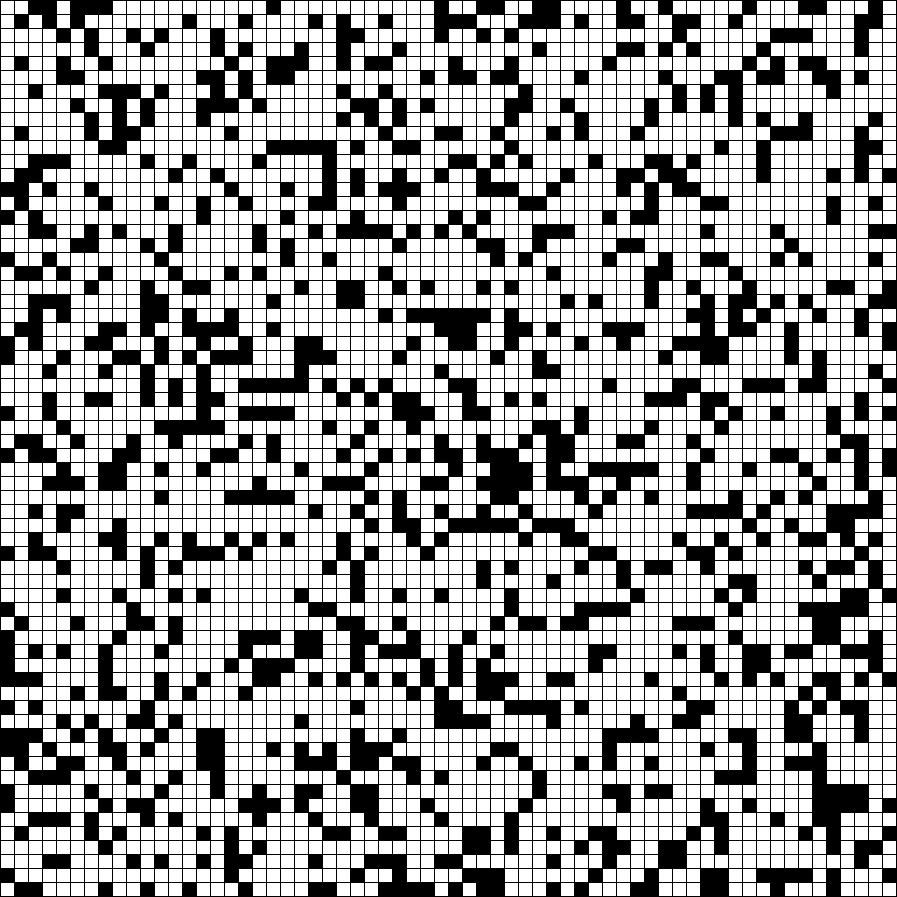
\includegraphics[scale=0.82]{images/m1.png}
    \caption{Uniform Random Fill Map}
    \label{fig: rep_Uniform Random Fill Map}
\end{figure}

\begin{table}[h!] 
\footnotesize
\centering


\begin{tabular}{|cc|c|c|c|c|c|}
\hline
\multicolumn{2}{|c|}{\textbf{Nr.}} & \textbf{Success Rate} & \textbf{Distance} & \textbf{Time} & \textbf{Distance Left}\\
\hline
\hline
\multicolumn{2}{|c|}{\cellcolor{lightgray!20} \hyperref[tab: evalalgorithms]{0}} & 100.0\% (I: 0\%) & 36.47 (A*: 36.47) (I: 0\%) & 0.0232s & 0.0\\
\hline
\hline
\multicolumn{2}{|c|}{\cellcolor{red!40} \hyperref[tab: evalalgorithms]{1}} & 44.0\% (I: -56.0\%) & 26.64 (A*: 25.8) (I: -3.26\%) & 0.0578s & 12.5\\
\hline
\multicolumn{2}{|c|}{\cellcolor{red!20} \hyperref[tab: evalalgorithms]{2}} & 6.0\% (I: -94.0\%) & 12.82 (A*: 11.71) (I: -9.48\%) & 0.0378s & 24.12\\
\hline
\multicolumn{2}{|c|}{\cellcolor{red!20} \hyperref[tab: evalalgorithms]{3}} & 24.0\% (I: -76.0\%) & 28.72 (A*: 23.69) (I: -21.23\%) & 0.0928s & 16.03\\
\hline
\multicolumn{2}{|c|}{\cellcolor{red!20} \hyperref[tab: evalalgorithms]{4}} & 50.0\% (I: -50.0\%) & 29.63 (A*: 28.64) (I: -3.46\%) & 0.0826s & 9.33\\
\hline
\multicolumn{2}{|c|}{\cellcolor{red!20} \hyperref[tab: evalalgorithms]{5}} & 44.0\% (I: -56.0\%) & 27.09 (A*: 25.92) (I: -4.51\%) & 0.0753s & 15.04\\
\hline
\hline
\multicolumn{2}{|c|}{\cellcolor{blue!20} \hyperref[tab: evalalgorithms]{6}} & 72.0\% (I: -28.0\%) & 35.29 (A*: 33.45) (I: -5.5\%) & 0.1295s & 8.02\\
\hline
\multicolumn{2}{|c|}{\cellcolor{blue!40} \hyperref[tab: evalalgorithms]{7}} & 8.0\% (I: -92.0\%) & 18.0 (A*: 15.78) (I: -14.07\%) & 0.0748s & 28.17\\
\hline
\multicolumn{2}{|c|}{\cellcolor{blue!20} \hyperref[tab: evalalgorithms]{8}} & 14.0\% (I: -86.0\%) & 31.79 (A*: 26.27) (I: -21.01\%) & 0.1017s & 18.97\\
\hline
\multicolumn{2}{|c|}{\cellcolor{blue!20} \hyperref[tab: evalalgorithms]{9}} & 42.0\% (I: -58.0\%) & 26.87 (A*: 25.79) (I: -4.19\%) & 0.0922s & 14.47\\
\hline
\multicolumn{2}{|c|}{\cellcolor{blue!20} \hyperref[tab: evalalgorithms]{10}} & 32.0\% (I: -68.0\%) & 23.15 (A*: 22.21) (I: -4.23\%) & 0.0972s & 14.94\\
\hline
\hline
\multicolumn{2}{|c|}{\cellcolor{orange!40} \hyperref[tab: evalalgorithms]{11}} & 74.0\% (I: -26.0\%) & 35.8 (A*: 33.71) (I: -6.2\%) & 1.1013s & 2.95\\
\hline
\hline
\multicolumn{1}{|M{0.15cm}}{\cellcolor{cyan!40}} & \multicolumn{1}{M{0.15cm}|}{\cellcolor{blue!40} \hspace*{-0.5cm}\hyperref[tab: evalalgorithms]{12}} & 100.0\% (I: 0\%) & 43.19 (A*: 36.47) (I: -18.43\%) & 0.5922s & 0.0\\
\hline
\multicolumn{1}{|M{0.15cm}}{\cellcolor{cyan!40}} & \multicolumn{1}{M{0.15cm}|}{\cellcolor{red!40} \hspace*{-0.5cm}\hyperref[tab: evalalgorithms]{13}} & 100.0\% (I: 0\%) & 38.23 (A*: 36.47) (I: -4.83\%) & 0.2458s & 0.0\\
\hline
\multicolumn{1}{|M{0.15cm}}{\cellcolor{cyan!40}} & \multicolumn{1}{M{0.15cm}|}{\cellcolor{orange!40} \hspace*{-0.5cm}\hyperref[tab: evalalgorithms]{14}} & 100.0\% (I: 0\%) & 39.79 (A*: 36.47) (I: -9.1\%) & 2.4698s & 0.0\\
\hline
\end{tabular}


\bigskip

\begin{tabular}{|cc|c|c|}
\hline
\multicolumn{2}{|c|}{\textbf{Nr.}} & \textbf{Pick Ratio}\\
\hline
\hline
\multicolumn{2}{|c|}{\cellcolor{orange!40} \hyperref[tab: evalalgorithms]{11}} & [4.0, 62.0, 8.0, 0.0, 4.0, 0.0, 0.0, 16.0, 4.0, 2.0]\%\\
\hline
\hline
\multicolumn{1}{|M{0.15cm}}{\cellcolor{cyan!40}} & \multicolumn{1}{M{0.15cm}|}{\cellcolor{orange!40} \hspace*{-0.5cm}\hyperref[tab: evalalgorithms]{14}} & [17.0, 64.33, 6.67, 3.67, 2.0, 0.0, 1.0, 4.33, 1.0, 0.0]\%\\
\hline
\end{tabular}


\bigskip

\begin{tabular}{|cc|c|c|c|c|M{3cm}|}
\hline
\multicolumn{2}{|c|}{\textbf{Nr.}} & \textbf{GK Improvement} & \textbf{GK Distance} & \textbf{GK Distance Left} & \textbf{WP} & \textbf{WP In-Between Distance}\\
\hline
\hline
\multicolumn{1}{|M{0.15cm}}{\cellcolor{cyan!40}} & \multicolumn{1}{M{0.15cm}|}{\cellcolor{blue!40} \hspace*{-0.5cm}\hyperref[tab: evalalgorithms]{12}} & 37.98\% & 15.05 & 25.22 & 7.12 & 2.64\\
\hline
\multicolumn{1}{|M{0.15cm}}{\cellcolor{cyan!40}} & \multicolumn{1}{M{0.15cm}|}{\cellcolor{red!40} \hspace*{-0.5cm}\hyperref[tab: evalalgorithms]{13}} & 65.87\% & 22.21 & 13.64 & 4.74 & 8.13\\
\hline
\multicolumn{1}{|M{0.15cm}}{\cellcolor{cyan!40}} & \multicolumn{1}{M{0.15cm}|}{\cellcolor{orange!40} \hspace*{-0.5cm}\hyperref[tab: evalalgorithms]{14}} & 97.61\% & 38.88 & 0.69 & 3.42 & 15.01\\
\hline
\end{tabular}


\bigskip

\begin{tabular}{|cc|c|c|c|c|c|}
\hline
\multicolumn{2}{|c|}{\textbf{Nr.}} & \textbf{Total Search} & \textbf{Total Fringe} & \textbf{Session Search} & \textbf{Session Fringe}\\
\hline
\hline
\multicolumn{2}{|c|}{\cellcolor{lightgray!20} \hyperref[tab: evalalgorithms]{0}} & 7.38\% & 2.34\% & 7.38\% & 2.34\%\\
\hline
\hline
\multicolumn{1}{|M{0.15cm}}{\cellcolor{cyan!40}} & \multicolumn{1}{M{0.15cm}|}{\cellcolor{blue!40} \hspace*{-0.5cm}\hyperref[tab: evalalgorithms]{12}} & 6.56\% (I: 11.11\%) & 2.34\% (I: 0\%) & 1.02\% (I: 86.18\%) & 0.4\% (I: 82.91\%)\\
\hline
\multicolumn{1}{|M{0.15cm}}{\cellcolor{cyan!40}} & \multicolumn{1}{M{0.15cm}|}{\cellcolor{red!40} \hspace*{-0.5cm}\hyperref[tab: evalalgorithms]{13}} & 5.24\% (I: 29.0\%) & 2.03\% (I: 13.25\%) & 1.17\% (I: 84.15\%) & 0.5\% (I: 78.63\%)\\
\hline
\multicolumn{1}{|M{0.15cm}}{\cellcolor{cyan!40}} & \multicolumn{1}{M{0.15cm}|}{\cellcolor{orange!40} \hspace*{-0.5cm}\hyperref[tab: evalalgorithms]{14}} & 4.69\% (I: 36.45\%) & 2.07\% (I: 11.54\%) & 1.43\% (I: 80.62\%) & 0.68\% (I: 70.94\%)\\
\hline
\end{tabular}


\caption{\textbf{Analyser} complex analysis on the uniform random fill map described in Figure \ref{fig: rep_Uniform Random Fill Map} with 50 random agent/goal positions}
\label{tab: eval_complex_analysis_map_1} 
\end{table}

\begin{itemize}
    \item Algorithm \hyperref[tab: evalalgorithms]{1} - same performance (the results are significantly worse than \cite{nicola2018lstm})
    \item Algorithm \hyperref[tab: evalalgorithms]{7} - has really bad performance as it has been trained on block maps and the uniform random fill map has a significantly different structure
    \item Algorithm \hyperref[tab: evalalgorithms]{11} - has worse success rate, same distance rate improvement and different picking pattern. The picking pattern is not well distributed and favours the algorithms which were trained on the uniform random fill map
    \item Algorithm \hyperref[tab: evalalgorithms]{14} - has a good kernel improvement and better distance improvement rate 
\end{itemize}

\pagebreak